\section{Decentralized search for \\ shortest path approximation}
\label{searching}

We propose to solve the point-to-point shortest path estimation problem using decentralized search with landmark based index. This section explain how decentralized search work with the index and underlying graph. Several aspects of the search including termination criterion, bidirectional search and tie breaking strategy are also discussed. 

\begin{figure*}[t]
    \centering
    \subfigure[Decentralized search]{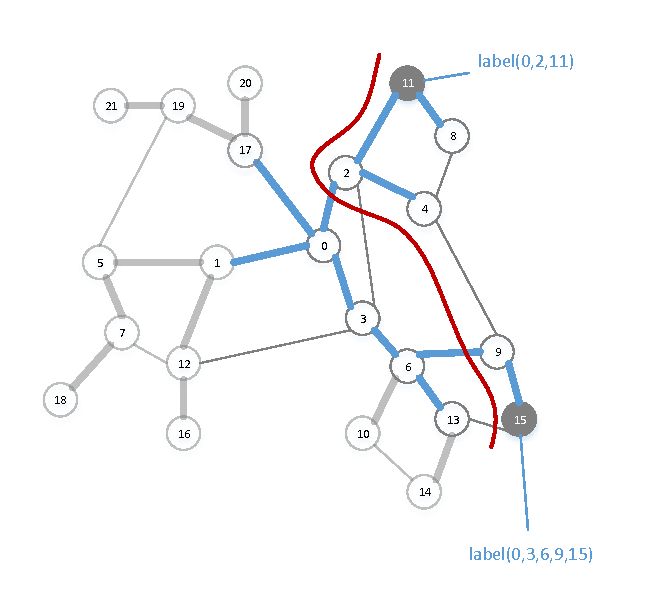
\epsfig{file=./figures/new_illustrate/dec_common.pdf,width=0.32\textwidth}}
    \subfigure[Bi-directional Decentralized Search]{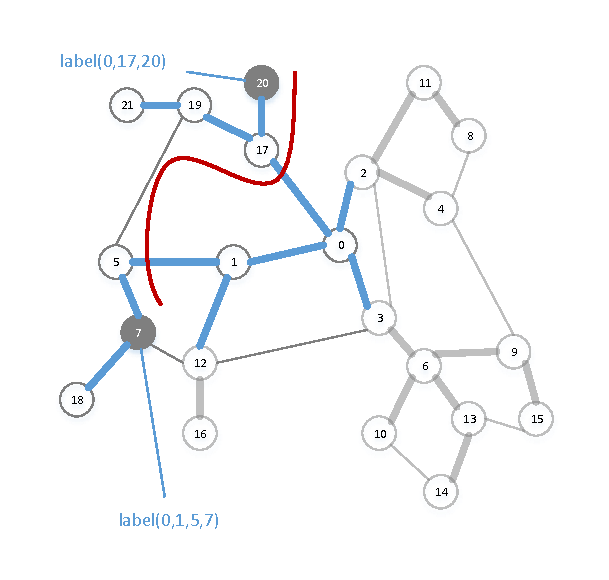
\epsfig{file=./figures/new_illustrate/bi_dec.pdf,width=0.32\textwidth}}
    \subfigure[Tie Strategy]{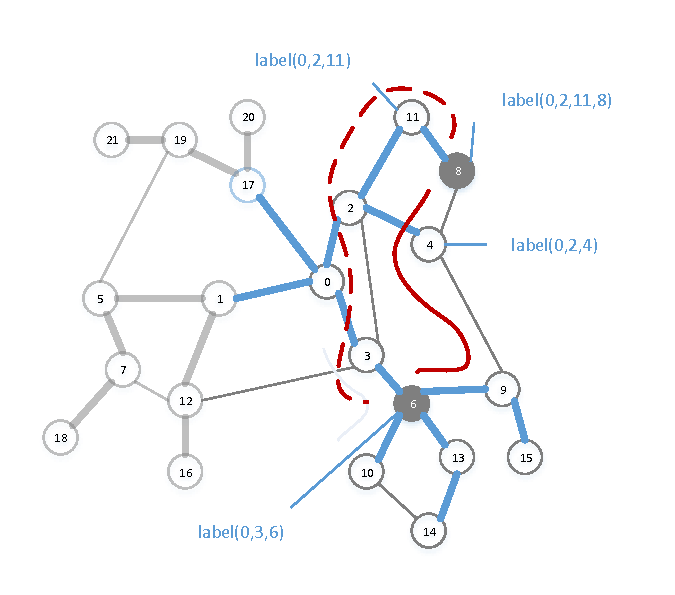
\epsfig{file=./figures/new_illustrate/tie.pdf,width=0.32\textwidth}}
    \caption{Cumulative distribution of the number of terminal nodes sampled by different algorithms.}
    \label{fig:cum_dis}
\end{figure*}

\subsection{Index guided decentralized search}

The decentralized search is performed on an indexed graph as follows. For a given pair of source and target vertex, the search start at the source vertex append it to the approximated path. The search examines each neighbor of vertex currently visited, for each neighbor, the LCA distance to the target vertex is calculated. The neighbor with least LCA distance will be picked as the vertex to visit next and append it to the approximated path. The search continues until it reach the target vertex. 

However, terminating when the search reaches the target vertex is a valid but not an ideal terminate criteria. Since the label of each vertex stores the shortest path of each vertex to each landmark. And shortest path follows the optimal substructure, i.e. the path between any two vertices along the shortest path is also the shortest path of them. So a search can stop once it  reaches any vertex in the label of the target vertex. The path contained in the label of target vertex is already the the shortest path due to the optimal substructure, we can directly concatenate it to the visited vertices to form a approximated path. 

The detailed algorithm of decentralized search is depicted in \ref{alg:dec}.

\begin{algorithm}
    \caption{Algorithm decentralized search}
		\label{alg:dec}
    \begin{algorithmic}
        \Function{DecentralizedSearch}{$G$, $s$, $t$}
					\State $p \gets \emptyset$
					\State $u \gets s$
					\State $p = p \cup u$
					\While{$u \notin L(t)$}
						\State $d_{min} \gets \infty$
						\State $w \gets u$
						\For{each $v$ adjecent to $u$}
							\If{$d_{LCA}(v,t) < d_{min}$}
								\State $d_{min} \gets d_{LCA}(V,t)$
								\State $w \gets v$ 
							\EndIf
						\EndFor
						\State $u \gets w$
						\State $p = p \cup u$
					\EndWhile
					\State $p_{remain} \gets$ path from $u$ to $t$ in $L(t)$ exclude $u$
					\State $p = p \cup p_{remain}$
					\State \Return $p$
        \EndFunction
    \end{algorithmic}
\end{algorithm}

At each step, by examining neighbor vertices the search is able to explore large part of the graph that is not included in the label of source and target vertex, which can potentially increase both accuracy and diversity of the path being found. For example in Fig. \ref{fig:dec_common} from $15$ to $11$, by following the procedure of decentralized search, instead of finding a short cut edge with both ends in labels of vertex $15$: $(0, 3, 6, 9, 15)$ and $11$: $(0, 2, 11)$, decentralized search can find a edge $(9, 4)$ that can lead to a shorter path which is denoted by solid curved line. 

So will the index guided decentralized search eventually terminate? As long as the source vertex $s$ and target vertex $t$ are reachable from each other, decentralized search will terminate in as much as ${\sigma}_{max}$ steps, where ${\sigma}_{max}$ is the diameter of the graph. To see this, first, the distance from $s$ to any vertex in $L(v)$ is shorter than ${\sigma}_{max}$. And at each step, suppose decentralized search is visiting vertex $u$, there must be a neighbor vertex $v$ that is on the path indicated by LCA computation of $u$ and $t$ that meet $d_{LCA}(v,t) \leq d_{LCA}(u,t) - 1$. Since decentralized search always pick the neighbor with least LCA distance to the target, the LCA distance to the target at each step will decrease at least by $1$. Therefore, decentralized search will terminate in at most ${\sigma}_{max}$ steps. 

The time complexity of Decentralized search depends on the max degree and the diameter of the graph. Decentralized search take at most ${\sigma}_{max}$ steps to finish. For each step, the search need to check at most ${\delta}_{max}$ neighbor vertices, where ${\delta}_{max}$ is the max vertex degree of the graph. For each neighbor, $k$ LCA computations are required where $k$ is the number of landmarks. The compuational time required for each LCA computation is $O(h)$ where $h$ is the height of the indexed shortest path tree. And we have $h \leq {\sigma}_{max}$ So the worst case time complexity of decentralized search is $O(k{{\sigma}_{max}}^2{\delta}_{max})$. 

The space complexity for decentralized search contains two parts, offline index space complexity and online query space complexity. The space required for offline index is $O(k{\sigma}_{max}n)$. For each query, $O(k{\sigma}_{max})$ space is required to store the labels of target vertex and the vertex that is being examined, $O({\sigma}_{max})$ space is required to store the approximated path. Combining them together, the online search space complexity of decentralized search is $O(k{\sigma}_{max})$.

\subsection{Bi-directional search}

In this section we show how to apply the idea of bidirectional search to decentralized search. In bidirectional decentralized search, the backward search starting at target vertex with a goal to reach the source vertex. Driven by a different goal and launched at a different start point, the backward search may explore a different search space compared to the forward search. It is not guaranteed that the forward search and backward search will eventually meet at any vertex except the source and target due to this difference. Actually, in decentralized search, the forward search and backward search are more like two independent search, that only resulting paths are required to be combined.

The main purpose for performing a backward search is to increase the possibility of finding a shorter approximate path and increase path diversity by exploring a different search space. This, however, is quiet different from the application of bidirectional search in BFS or A* search where the main focus is to reduce search space. For example in Fig. \ref{fig:bi_dec}, the search starts from $20$ to $7$ can find a shorter path $p = (20, 17, 19, 5, 7)$ than the search starts at $7$. Due to that $0$ has a smaller LCA distance to $7$ than $19$, the edge $(19, 5)$ cannot be found by the search starts from $20$. 

\subsection{Handle ties}

Tie happens frequently in decentralized search, especially when the number of landmarks is small. A tie here means during decentralized search, there are multiple neighbors of a visited vertex that have same LCA distance to the target. The reason for tie is that there is not sufficient information in the index that can separate some vertices for a query. For example in Fig. \ref{fig:tie}, to find path from $8$ to $6$, when traversing neighbors of vertex $8$, both vertex $11$ and $4$ have the same LCA distance to vertex $6$, but their actual distances to vertex $6$ are different due to edges currently invisible to the decentralized search. Note that tie is always query-dependent, different queries may have very different tie patterns even if the related searches examine similar search spaces. 

Expanding the search onto each tie vertex require the search examine different sets of vertices and edges which increase the cost of the search, but also increase the chance to find a shorter path as well. Two obvious solution to deal with ties are either randomly pick one vertex to visit or visit all vertices in the next step. The former one incur no additional cost and will have the least possibility to find a shorter path, we refer to it as single branch decentralized search. The latter one require most effort and will lead to the shortest path the decentralized search could possibly find, we refer to it as full branch decentralized search.

[k branch] The single branch decentralized search and full branch decentralized search define the achievable accuracy range of decentralized search. The number of ties during on complex networks also follows a power-law distribution.
